\documentclass[12pt,a4paper]{article}
\usepackage[utf8]{inputenc} % For UTF-8 encoding
\usepackage[T1]{fontenc} % For T1 font encoding
\usepackage{graphicx} % For including images
\usepackage{geometry} % For setting page margins
\usepackage{setspace} % For setting line spacing
\usepackage{booktabs} % For better table formatting
\usepackage{multirow} % For multi-row cells in tables
\usepackage{hyperref} % For hyperlinks
\usepackage{float}    % already used for precise float control
\usepackage{placeins} % add this line to enforce float barriers
\usepackage{listings} % For code listings
\usepackage{xcolor} % For colored text

\lstset{
  basicstyle=\ttfamily\small,
  breaklines=true,
  commentstyle=\color{green!50!black},
  keywordstyle=\color{blue},
  stringstyle=\color{red},
  numbers=left,
  numberstyle=\tiny\color{gray},
  numbersep=5pt,
  frame=single,
  framesep=5pt
}

\geometry{
    top=1.5cm,
    bottom=1.5cm,
    left=1.5cm,
    right=1.5cm
}

\begin{document}
\begin{titlepage}
    \begin{minipage}{0.15\textwidth}
        
\includegraphics[width=\linewidth]{university-logo.png}
    \end{minipage}
    \begin{minipage}{0.625\textwidth}
        \centering
        \MakeUppercase{
            Université Abdelhamidhri Constantine 2\\
            Faculté des Nouvelles Technologies de l'Information et de la Communication NTIC\\
            Le Département Technologies des Logiciels et des Systèmes d'Information TLSI
        }
    \end{minipage}
    \begin{minipage}{0.15\textwidth}
        
\includegraphics[width=\linewidth]{ntic-logo.png}
    \end{minipage}
    
    \vspace{3cm}

    \begin{center}
        \LARGE{\textbf{TP MEL \\ rapport 2}}
    \end{center}

    \vspace{0.1cm}

    \begin{center}
        SPECIALTY: SOFTWARE ENGINEERING
    \end{center}
    
    \vspace{1.9cm}
    \hrule
    \vspace{0.5cm}

    \begin{center}
        \LARGE{\textbf{Maintenance of DAC Project (overView)}}
    \end{center}
    
    \vspace{0.5cm}
    \hrule
    \vspace{2cm}
    
    \begin{minipage}[t]{0.66\textwidth}
        \textbf{Supervised by:}\\
        • Dr. Manel DJENOUHAT
    \end{minipage}
    \hfill
    \begin{minipage}[t]{0.4\textwidth}
        \textbf{Presented by:}\\
        • Rouissa Rabah G2\\
        • Belmokhi Dibadj G2\\
        • Brahmia Mohamed\\Haythem Abderrahmen G2
    \end{minipage}

    \vspace{5cm}

    \begin{center}
        \large\textbf{DATE: 17/03/2025}
    \end{center}
\end{titlepage}

\thispagestyle{empty}
\tableofcontents
\newpage
\thispagestyle{empty}
\listoftables
\newpage
\thispagestyle{empty}
\listoffigures
\newpage
\pagenumbering{arabic}

\section{Introduction}
\subsection{Project Context}
SORTVIEW Desktop Application project focuses on creating a high-performance, user-friendly tool 
that enables users to classify multiple images concurrently. The application will allow users to load and 
display images, initiate classification tasks. Leveraging multi-threading, it will support simultaneous 
processing to optimize performance and efficiency. Robust error-handling mechanisms will ensure the 
application functions smoothly. The project emphasizes simplicity, clarity, and usability in its interface 
design, ensuring a seamless user experience. 
\subsection{Maintenance Objectives}
The primary objectives for maintaining the SORTVIEW Desktop Application are:

\subsubsection{Code Understandability}
Ensure that the code is easy to understand for future developers. This will be achieved by fixing variable names, using clear and consistent naming conventions, and removing any ambiguities that may lead to misunderstandings.

\subsubsection{Eliminating Code Duplication}
Address any instances of duplicated code to reduce redundancy and make the code more maintainable. This will ensure that changes are easier to implement and less error-prone.

\subsubsection{Optimizing Code}
Remove unnecessary or overly complicated lines of code to improve efficiency. Refactor complex logic into simpler, more modular components to improve readability and maintainability.
\subsection{Tools and Methodology}
For efficient maintenance, the following tools and methodologies will be used:

\subsubsection{SonarCloud}
The primary focus will be on using SonarCloud for continuous static code analysis to identify and fix code smells. This will help in eliminating unnecessary complexities, improving code readability, and ensuring that the code remains easy to maintain for future developers.
\subsubsection{GitHub}
GitHub will be used for version control, enabling smooth collaboration, tracking changes, and managing code history. It ensures that all modifications are well-documented and easy to access by future developers.

By prioritizing the resolution of code smells and minimizing unnecessary complexity, the SORTVIEW Desktop Application will remain clean, understandable, and easier for future developers to maintain while preserving its core functionality.

\section{Analysis of Current State}
\subsection{SonarQube Metrics Overview}
\begin{figure}[H]
    \centering
    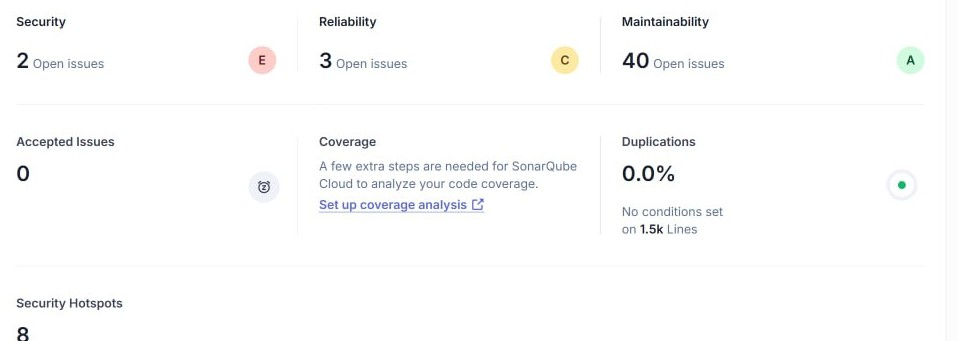
\includegraphics[width=1\textwidth]{SonarQube Metrics Overview.jpg}
    \caption{SonarQube Metrics Overviewe}
    \label{fig:SMO}
\end{figure}

\section{Identified Issues}
\subsection{Security Issues}
\begin{figure}[H]
    \centering
    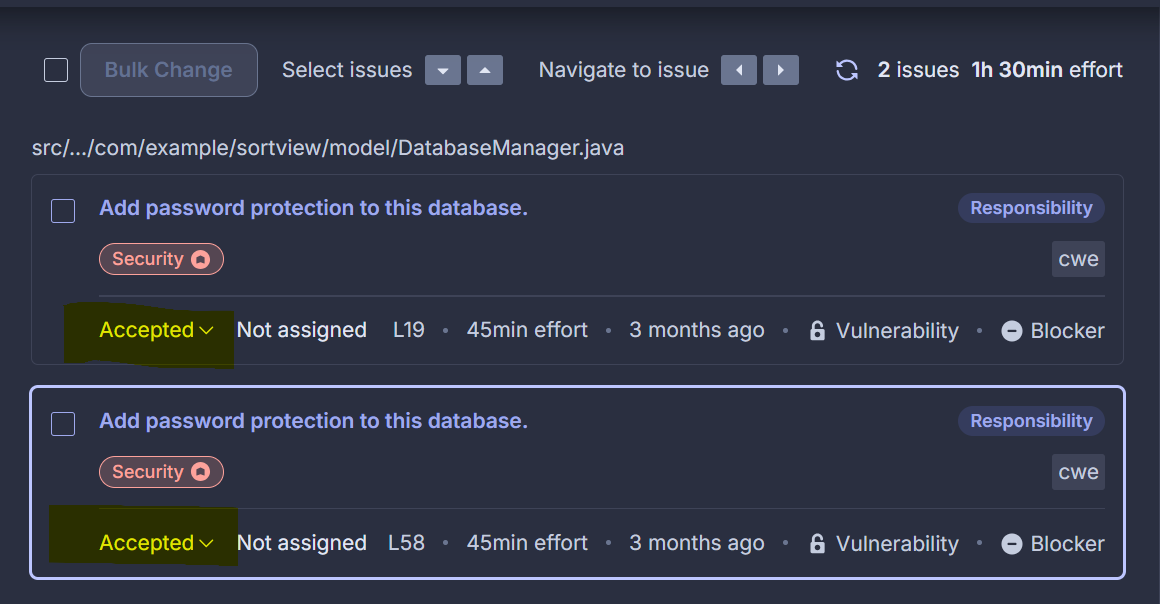
\includegraphics[width=1\textwidth]{Security Issues.png}
    \caption{Security Issues}
    \label{fig:SI}
\end{figure}
\subsection{Reliability Issues}
\begin{figure}[H]
    \centering
    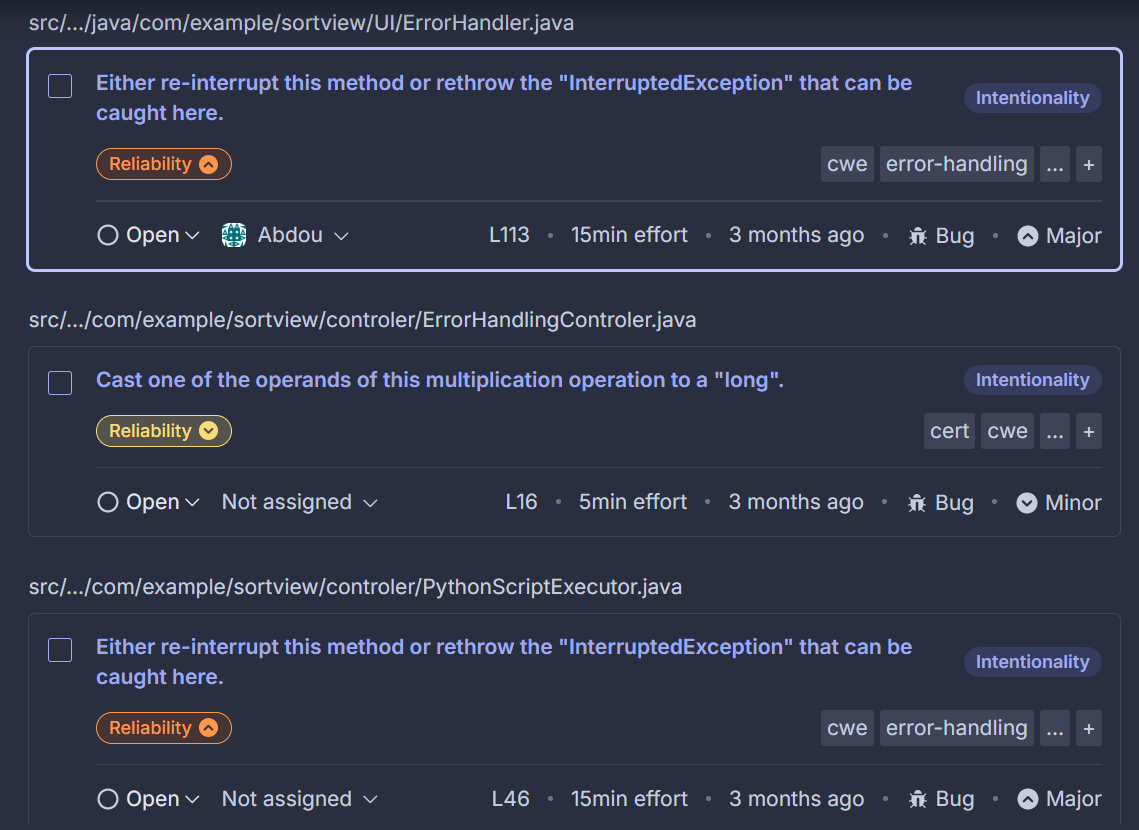
\includegraphics[width=1\textwidth]{Reliability Issues-3I.png}
    \caption{Reliability Issues Overview}
    \label{fig:3I}
\end{figure}
\begin{figure}[H]
    \centering
    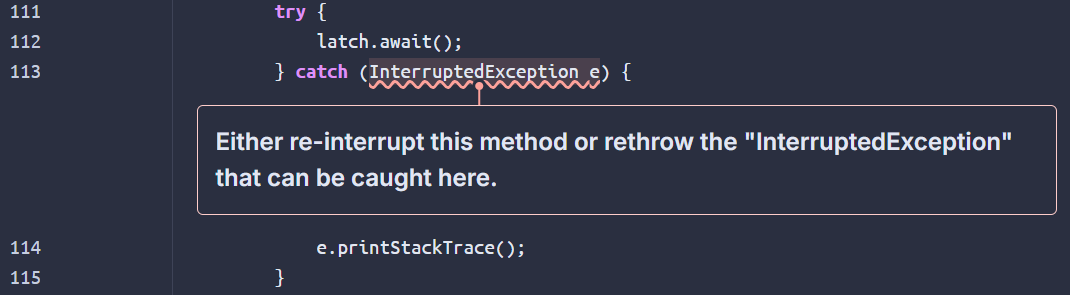
\includegraphics[width=1\textwidth]{Reliability Issues-1st.png}
    \caption{Reliability Issues - First Issue}
    \label{fig:1st}
\end{figure}
\begin{figure}[H]
    \centering
    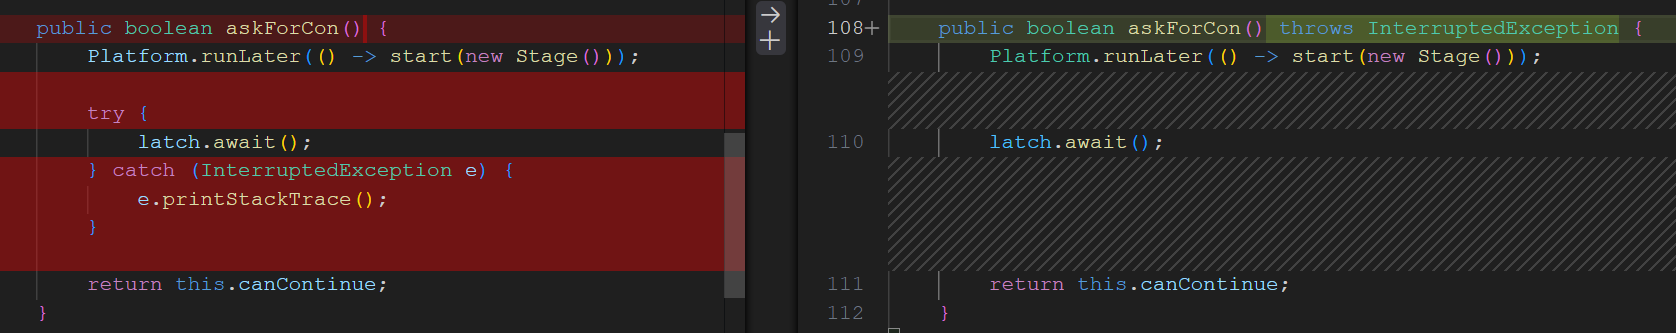
\includegraphics[width=1\textwidth]{Reliability Issues-1stS.png}
    \caption{Reliability Issues - First Issue Solution}
    \label{fig:1stS}
\end{figure}
\begin{figure}[H]
    \centering
    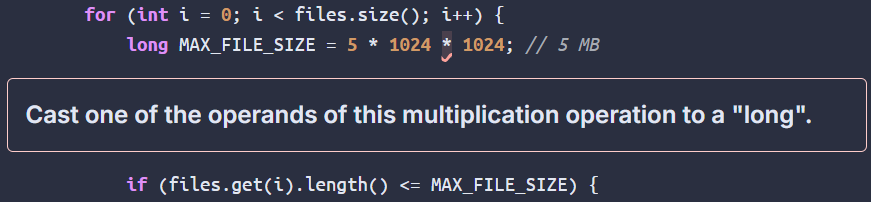
\includegraphics[width=1\textwidth]{Reliability Issues-2nd.png}
    \caption{Reliability Issues - Second Issue}
    \label{fig:2nd}
\end{figure}
\begin{figure}[H]
    \centering
    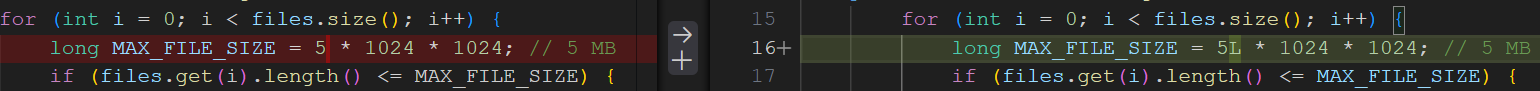
\includegraphics[width=1\textwidth]{Reliability Issues-2ndS.png}
    \caption{Reliability Issues - Second Issue Solution}
    \label{fig:2ndS}
\end{figure}
\begin{figure}[H]
    \centering
    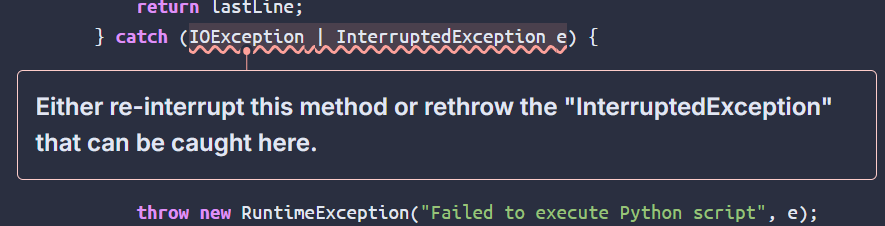
\includegraphics[width=1\textwidth]{Reliability Issues-3rd.png}
    \caption{Reliability Issues - Third Issue}
    \label{fig:3rd}
\end{figure}
\begin{figure}[H]
    \centering
    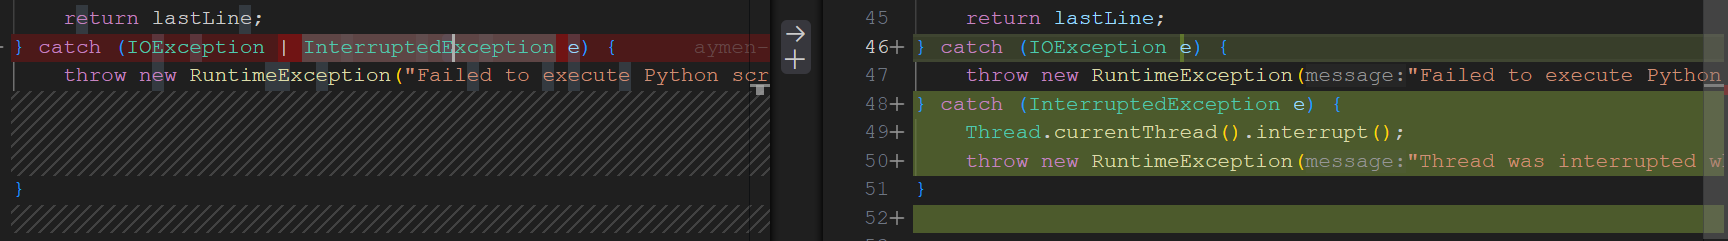
\includegraphics[width=1\textwidth]{Reliability Issues-3rdS.png}
    \caption{Reliability Issues - Third Issue Solution}
    \label{fig:3rdS}
\end{figure}


\subsection{Maintinability Issues}
\begin{figure}[H]
    \centering
    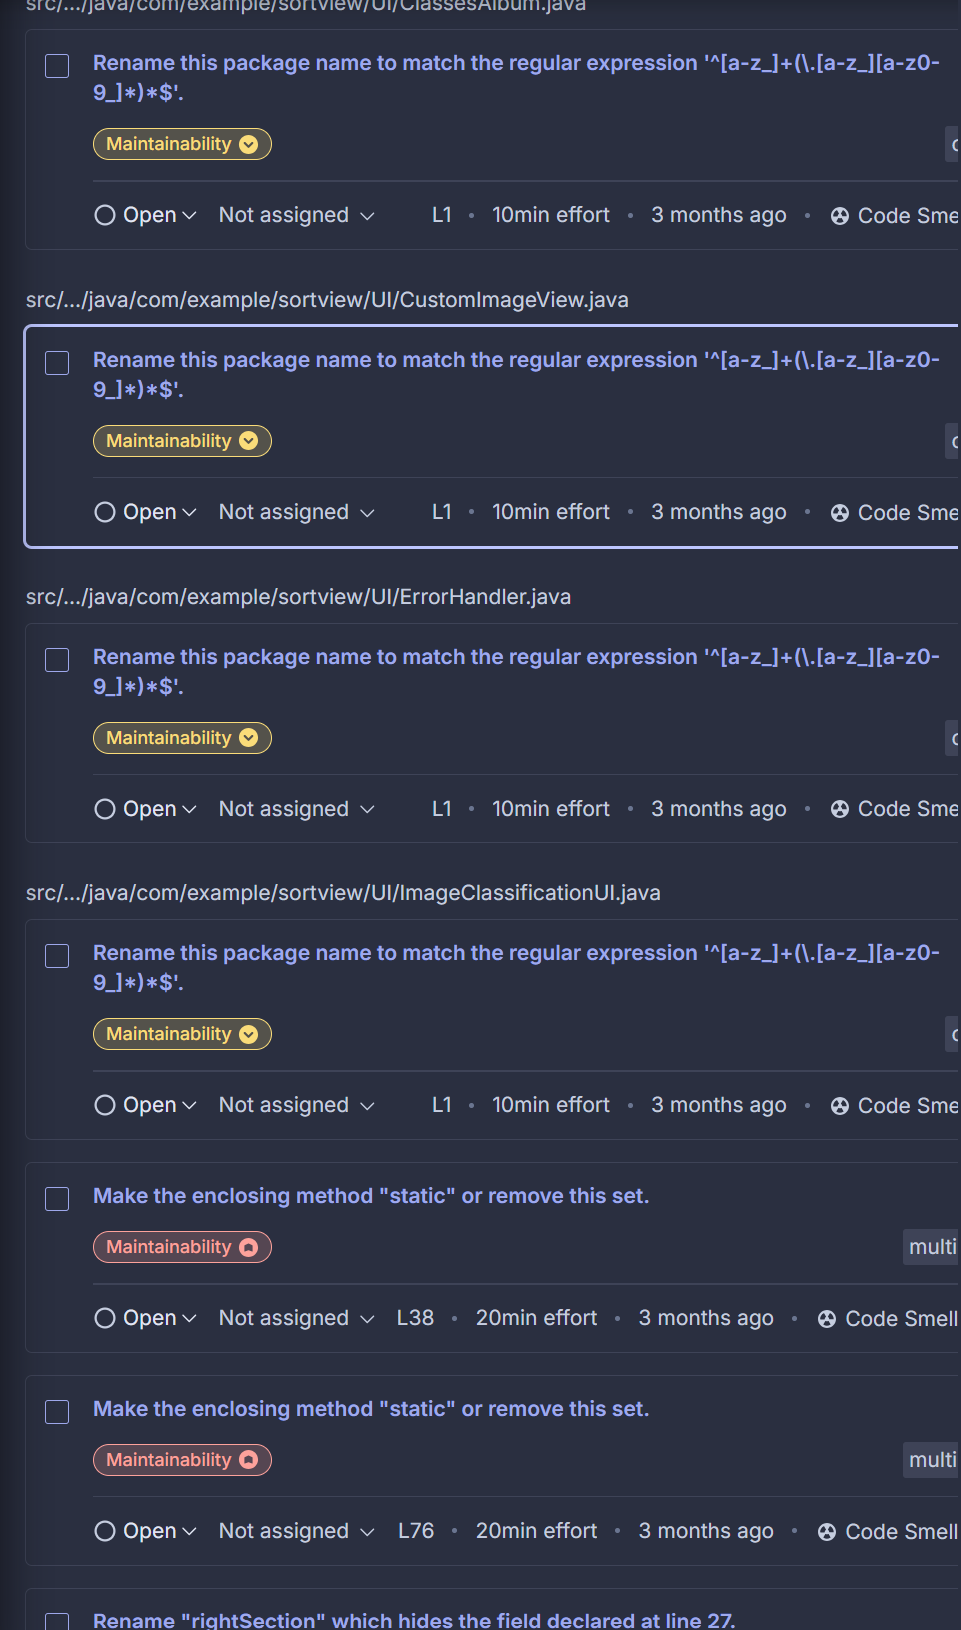
\includegraphics[width=0.8\textwidth]{Maintainability Issues-40I.png}
    \caption{Maintainability Issues Overview}
    \label{fig:40I}
\end{figure}
\begin{figure}[H]
    \centering
    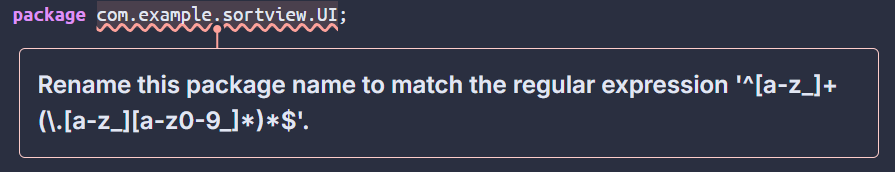
\includegraphics[width=1\textwidth]{Maintainability Issues-1st.png}
    \caption{Maintainability Issues - First Issue}
    \label{fig:MI-1st}
\end{figure}
\begin{figure}[H]
    \centering
    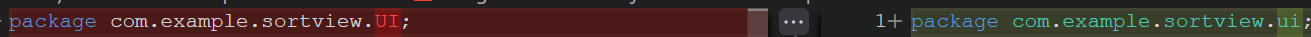
\includegraphics[width=1\textwidth]{Maintainability Issues-1stS.png}
    \caption{Maintainability Issues - First Issue Solution}
    \label{fig:MI-1stS}
\end{figure}
\begin{figure}[H]
    \centering
    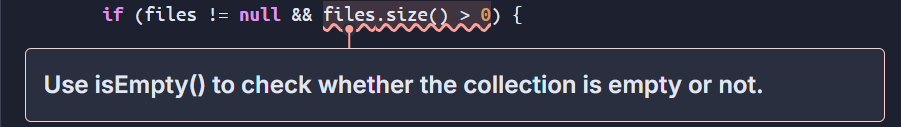
\includegraphics[width=1\textwidth]{Maintainability Issues-2nd.png}
    \caption{Maintainability Issues - Second Issue}
    \label{fig:MI-2nd}
\end{figure}
\begin{figure}[H]
    \centering
    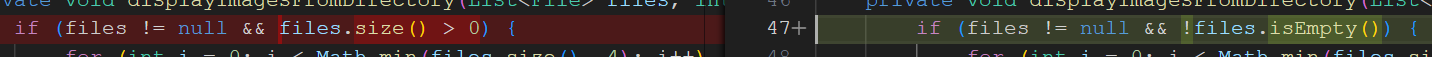
\includegraphics[width=1\textwidth]{Maintainability Issues-2ndS.png}
    \caption{Maintainability Issues - Second Issue Solution}
    \label{fig:MI-2ndS}
\end{figure}
\begin{figure}[H]
    \centering
    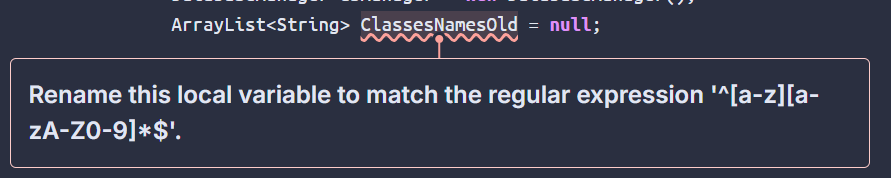
\includegraphics[width=1\textwidth]{Maintainability Issues-3rd.png}
    \caption{Maintainability Issues - Third Issue}
    \label{fig:MI-3rd}
\end{figure}
\begin{figure}[H]
    \centering
    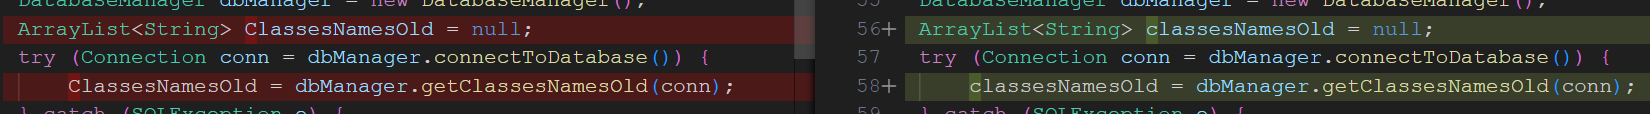
\includegraphics[width=1\textwidth]{Maintainability Issues-3rdS.png}
    \caption{Maintainability Issues - Third Issue Solution}
    \label{fig:MI-3rdS}
\end{figure}
\begin{figure}[H]
    \centering
    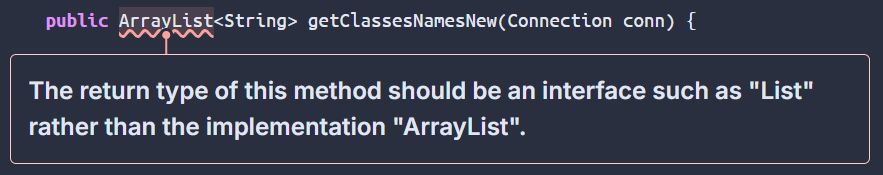
\includegraphics[width=1\textwidth]{Maintainability Issues-4th.png}
    \caption{Maintainability Issues - Fourth Issue}
    \label{fig:MI-4th}
\end{figure}
\begin{figure}[H]
    \centering
    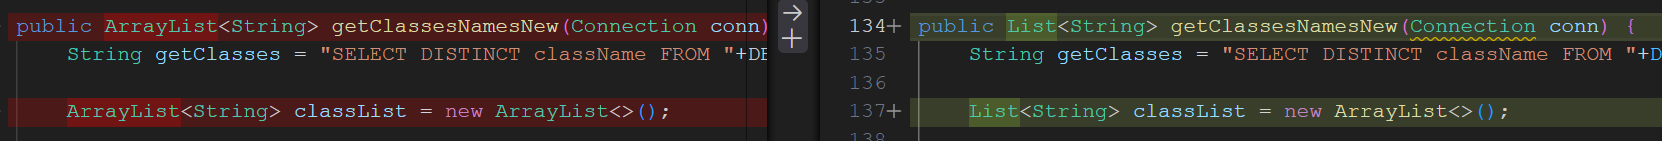
\includegraphics[width=1\textwidth]{Maintainability Issues-4thS.png}
    \caption{Maintainability Issues - Fourth Issue Solution}
    \label{fig:MI-4thS}
\end{figure}
\begin{figure}[H]
    \centering
    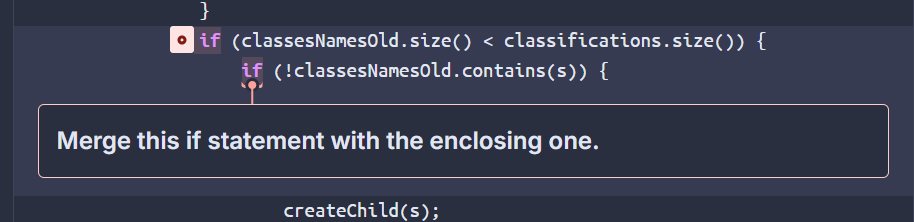
\includegraphics[width=1\textwidth]{Maintainability Issues-5th.png}
    \caption{Maintainability Issues - Fifth Issue}
    \label{fig:MI-5th}
\end{figure}
\begin{figure}[H]
    \centering
    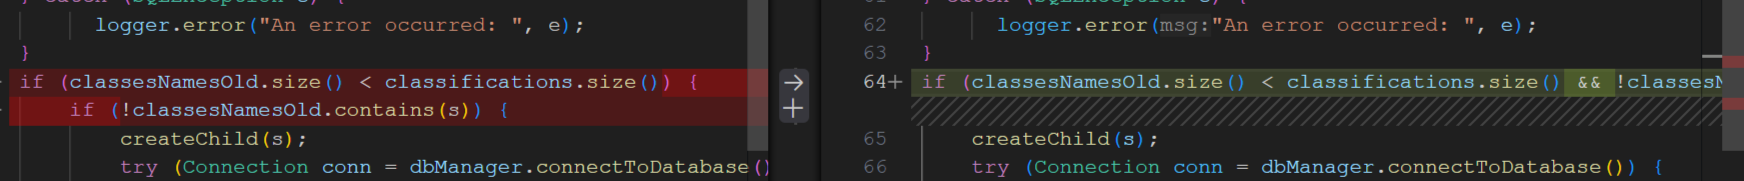
\includegraphics[width=1\textwidth]{Maintainability Issues-5thS.png}
    \caption{Maintainability Issues - Fifth Issue Solution}
    \label{fig:MI-5thS}
\end{figure}
\begin{figure}[H]
    \centering
    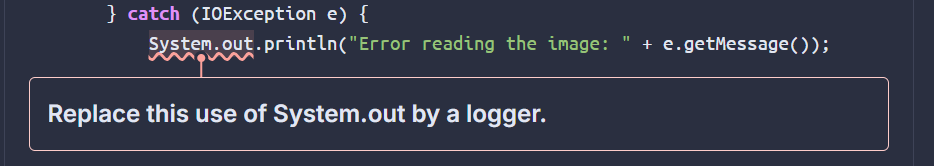
\includegraphics[width=1\textwidth]{Maintainability Issues-6th.png}
    \caption{Maintainability Issues - Sixth Issue}
    \label{fig:MI-6th}
\end{figure}
\begin{figure}[H]
    \centering
    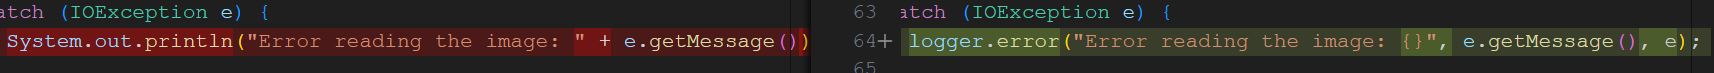
\includegraphics[width=1\textwidth]{Maintainability Issues-6thS.png}
    \caption{Maintainability Issues - Sixth Issue Solution}
    \label{fig:MI-6thS}
\end{figure}
\subsection{Security Hotspots}
\begin{figure}[H]
    \centering
    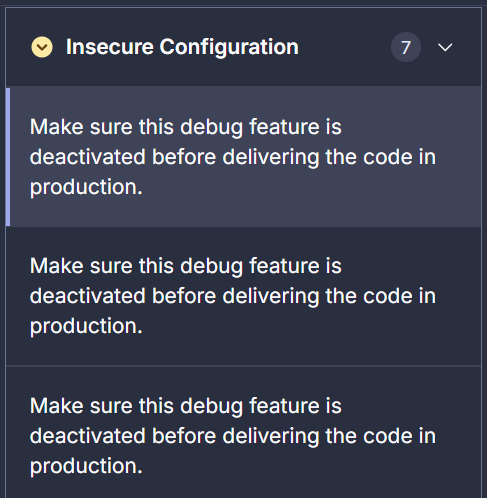
\includegraphics[width=1\textwidth]{Security Hotspots-7i.png}
    \caption{Security Hotspots Overview}
    \label{fig:7I}
\end{figure}
\begin{figure}[H]
    \centering
    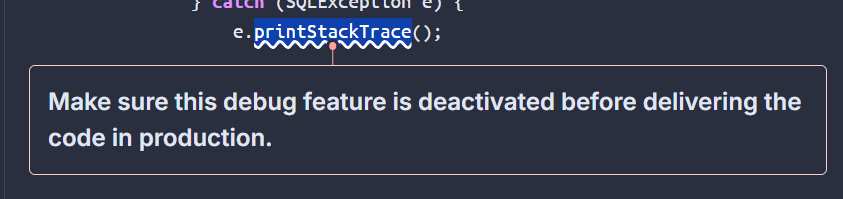
\includegraphics[width=1\textwidth]{Security Hotspots-1st.png}
    \caption{Security Hotspots - First Issue}
    \label{fig:SH-1st}
\end{figure}
\begin{figure}[H]
    \centering
    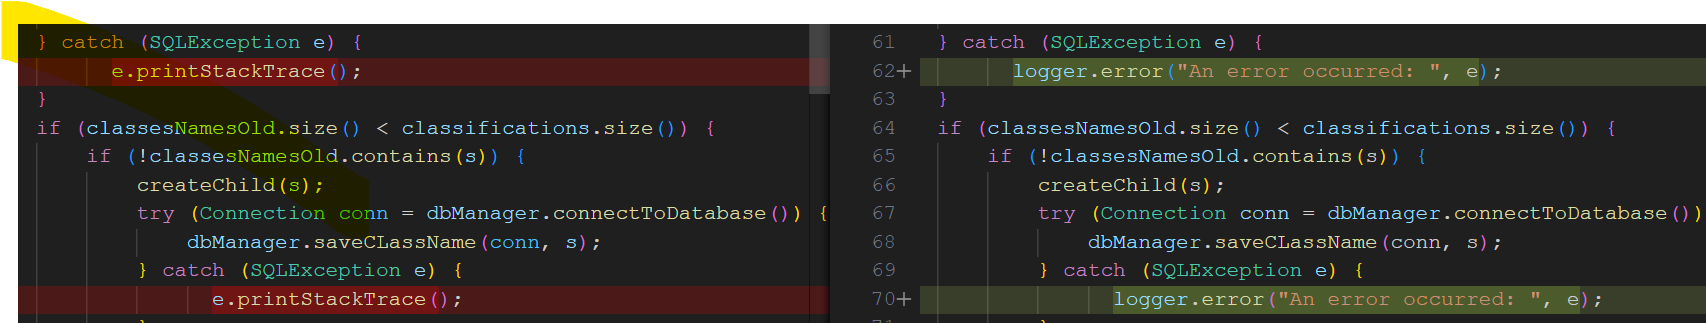
\includegraphics[width=1\textwidth]{Security Hotspots-1stS.png}
    \caption{Security Hotspots - First Issue Solution}
    \label{fig:SH-1stS}
\end{figure}

\section{Results and Verification}
\subsection{SonarQube Results After Maintenance}

\begin{figure}[H]
    \centering
    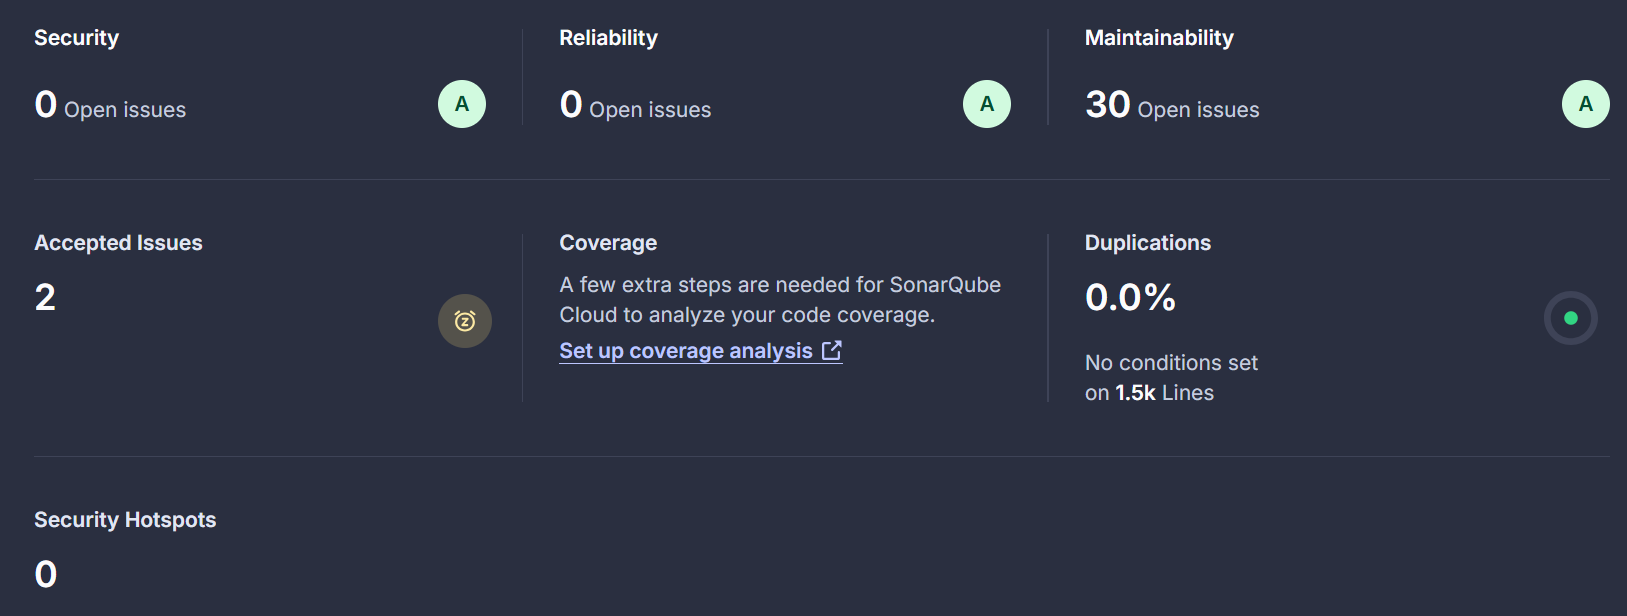
\includegraphics[width=1\textwidth]{SonarQube Metrics Overview-A.jpg.png}
    \caption{SonarQube Metrics Overview After Maintenance}
    \label{fig:SMO-A}
\end{figure}

\begin{table}[H]
\centering
\begin{tabular}{lcc}
\toprule
\textbf{Metric} & \textbf{Before} & \textbf{After} \\ 
\midrule
Security Issues & 2 & 0 \\ 
Reliability Issues & 3 & 0 \\ 
Maintainability Issues & 40 & 30 \\ 
Accepted Issues & 0 & 2 \\ 
Coverage & Not configured & Not configured \\ 
Duplications & 0.0\% & 0.0\% \\ 
Security Hotspots & 8 & 0 \\ 
\bottomrule
\end{tabular}
\caption{SonarQube Analysis Results - Before vs. After}
\end{table}

\end{document}

